\chapter{Friction}

Imagine there is a large and heavy steel box resting in the middle of a large floor   Imagine you push it hard enough to get it moving.   If you stop pushing,  will it continue to glide gracefully across the floor? 

Probably not.  Unless the floor is very slippery for some reason,  the box will come to a halt immediately after you stop pushing.  We would say that it is stopped by the force of \newterm{friction}. 

What's really happening?  The kinetic energy of the box is being converted into heat 
between the bottom of the box and floor.   As the bottom of the box and the floor get warmer,  the speed of the box decreases.

The amount of friction is proportional to the force with which the box is pressing against the floor -- so you should expect a box that is twice as heavy to experience twice as much frictional force.

That is,  the frictional force is proportional to the normal force.  (FIXME: picture here)

The amount of friction is also determined by the materials that are sliding against each other.  For example,  if the floor is ice,  the frictional force will be less than if the floor is made of wood. 

If you are pushing the box with a force of $F$ and it is moving but neither accelerating nor decelerating,  then the force you are applying is exactly balanced by the frictional force.  If the box is pressing against the floor with a force of $N$, then we say the \newterm{coefficient of friction} between the steel box and the floor is given by

$$\mu = \frac{F}{N}$$

\begin{Exercise}[title={Bicycle Stopping},  label=bike_stop]
  
You are riding your bicycle at 11 meters per second when you slam on the brakes and lock up the wheels.  

You weigh 55 kg.   

When any piece of rubber is skidding across a dry road,  the coefficient of friction will be about 0.7.

Answer the following questions: 

\begin{itemize}
\item How much kinetic energy do you have when you engage the brakes?
\item As you skid,  how much frictional force is decelerating you?
\item For how many meters will you slide?
\end{itemize}

\end{Exercise}
\begin{Answer}[ref=bike_stop]

Kinetic energy? $E = mv^2 = (55)(11^2) = 6,655 \frac{kg m^2}{s^2} = 6,655$ joules.

Frictional force? $F = \mu N = (0.7)(55)(9.8) = 377.3$ newtons.

Distance?  $D = \frac{6,655}{377.3} = 17.6$ seconds.

\end{Answer}

Notice that the force of friction is not determined by how much of the tire is touching the ground.  The coefficient of friction of the two materials and the normal force all all you need to compute the friction.

\section{Static vs Kinetic Friction Coefficients}

Once again, imagine the box resting on the floor.  As you start to push it,  it will sit still until your force is greater than the force of friction.   However, once it starts moving,  the force of friction seems to be less.

Between two materials,  there is actually 2 different friction coefficients:

\begin{itemize}
\item Kinetic friction coefficient:  The coefficient you use once the box is sliding against the floor.
\item Static friction coefficient: The coefficient you use to figure out how much force you need to get the box to start to move.
\end{itemize}

The kinetic friction coefficient is always less than the static friction coefficient:
\begin{itemize}
\item \textit{Kinetic}, $\mu_k$: For a car skidding on a dry road,  the friction coefficient is about 0.7.  
\item \textit{Static}, $\mu_s$: When the car is parked with its brakes on,  it has a friction coefficient of about 1.0.
\end{itemize}

\begin{Exercise}[title={Rocket Sled},  label=rocketsled1]
  
You are built a rocket sled with steel runners on a flat, level wooden floor.   The sled weighs 50 kg and you weigh 55 kg.

Before you get on the sled,   you push it around the floor some.  You find that you can get it to move from a
standstill if you push it with a force of 270 N.   Once it is moving,  you can keep it moving at the same speed using a force of 220 N.

\textbf{What are $\mu_s$ and $\mu_k$  of your sled's runners on your wooden floor?}

Now you get on the sled and gradually increase the thrust of the rocket mounted on the sled until it starts to move.  Then you keep the thrust constant.

\textbf{How much force was the rocket exerting on you and the sled when it started to move?}

\textbf{How how fast do you accelerate now that the sled is moving?}

\end{Exercise}
\begin{Answer}[ref=rocketsled1]

The empty sled is pushing directly down on the floor with a force of $(50)(9.8) = 490$ N.

The force to overcome the static friction  is:

$$270 = 490 \mu_s$$

Thus $\mu_s = 0.551$

The force to match kinetic friction is:

$$220 = 490 \mu_k$$

Thus $\mu_k = 0.449$

Once you are on the sled,  it is pressing directly down on the floor with a force of $(50  + 55)(9.8) = 1,029$ N.

The force to overcome the static friction is:

$$F = (1,029)(0.551) = 567 \text{ N}$$

Once the sled is moving,  friction is counteracting some of your force.  How much?

$$F_f = (1,029)(0.449) = 462 \text{ N}$$

So all of your acceleration is due to the remaining $567 - 492 = 75$ N.

We know that $F = ma$.  In this case $F = 75$ N and $m = 105$ kg.  So

$$a = \frac{75}{105} = 0.714 \text{ meters per second per second}$$

\end{Answer}

\section{Skidding and Anti-Lock Braking Systems}

When a car goes through a curve,  the friction of the tire on the road is what changes the direction of the 
car's travel.  Even though the wheel is turning,   this is the static friction coefficient because the surface of the tire is not sliding across the road.

If you go into the curve too fast,  the tire may not have enough friction to turn the car.  In this case the car will start to slide sideways.  Now the friction between the tire and road uses the kinetic coefficient.  That is,   you have significantly less friction than you had before you started to skid.

When you are driving a car,  the force of friction that your tires create is your friend.  It lets you steer, accelerate, and stop.

In older cars,  if you would panicked  and slammed on the brakes,  you would probably lock up the wheels: they would stop turning suddenly.  And the surface of the tire would begin to slide across the pavement.  At that moment,  two problems occurred:
\begin{itemize}
\item You don't stop as quickly because now the friction between your tires and the road is based on the kinetic friction coefficient instead of the static friction coefficient.
\item You can't steer the car.  Steering only happens because the wheels are turning in a particular direction.
\end{itemize}

To prevent this problem,  car companies developed the anti-lock brake system or ABS.

FIXME: More here.

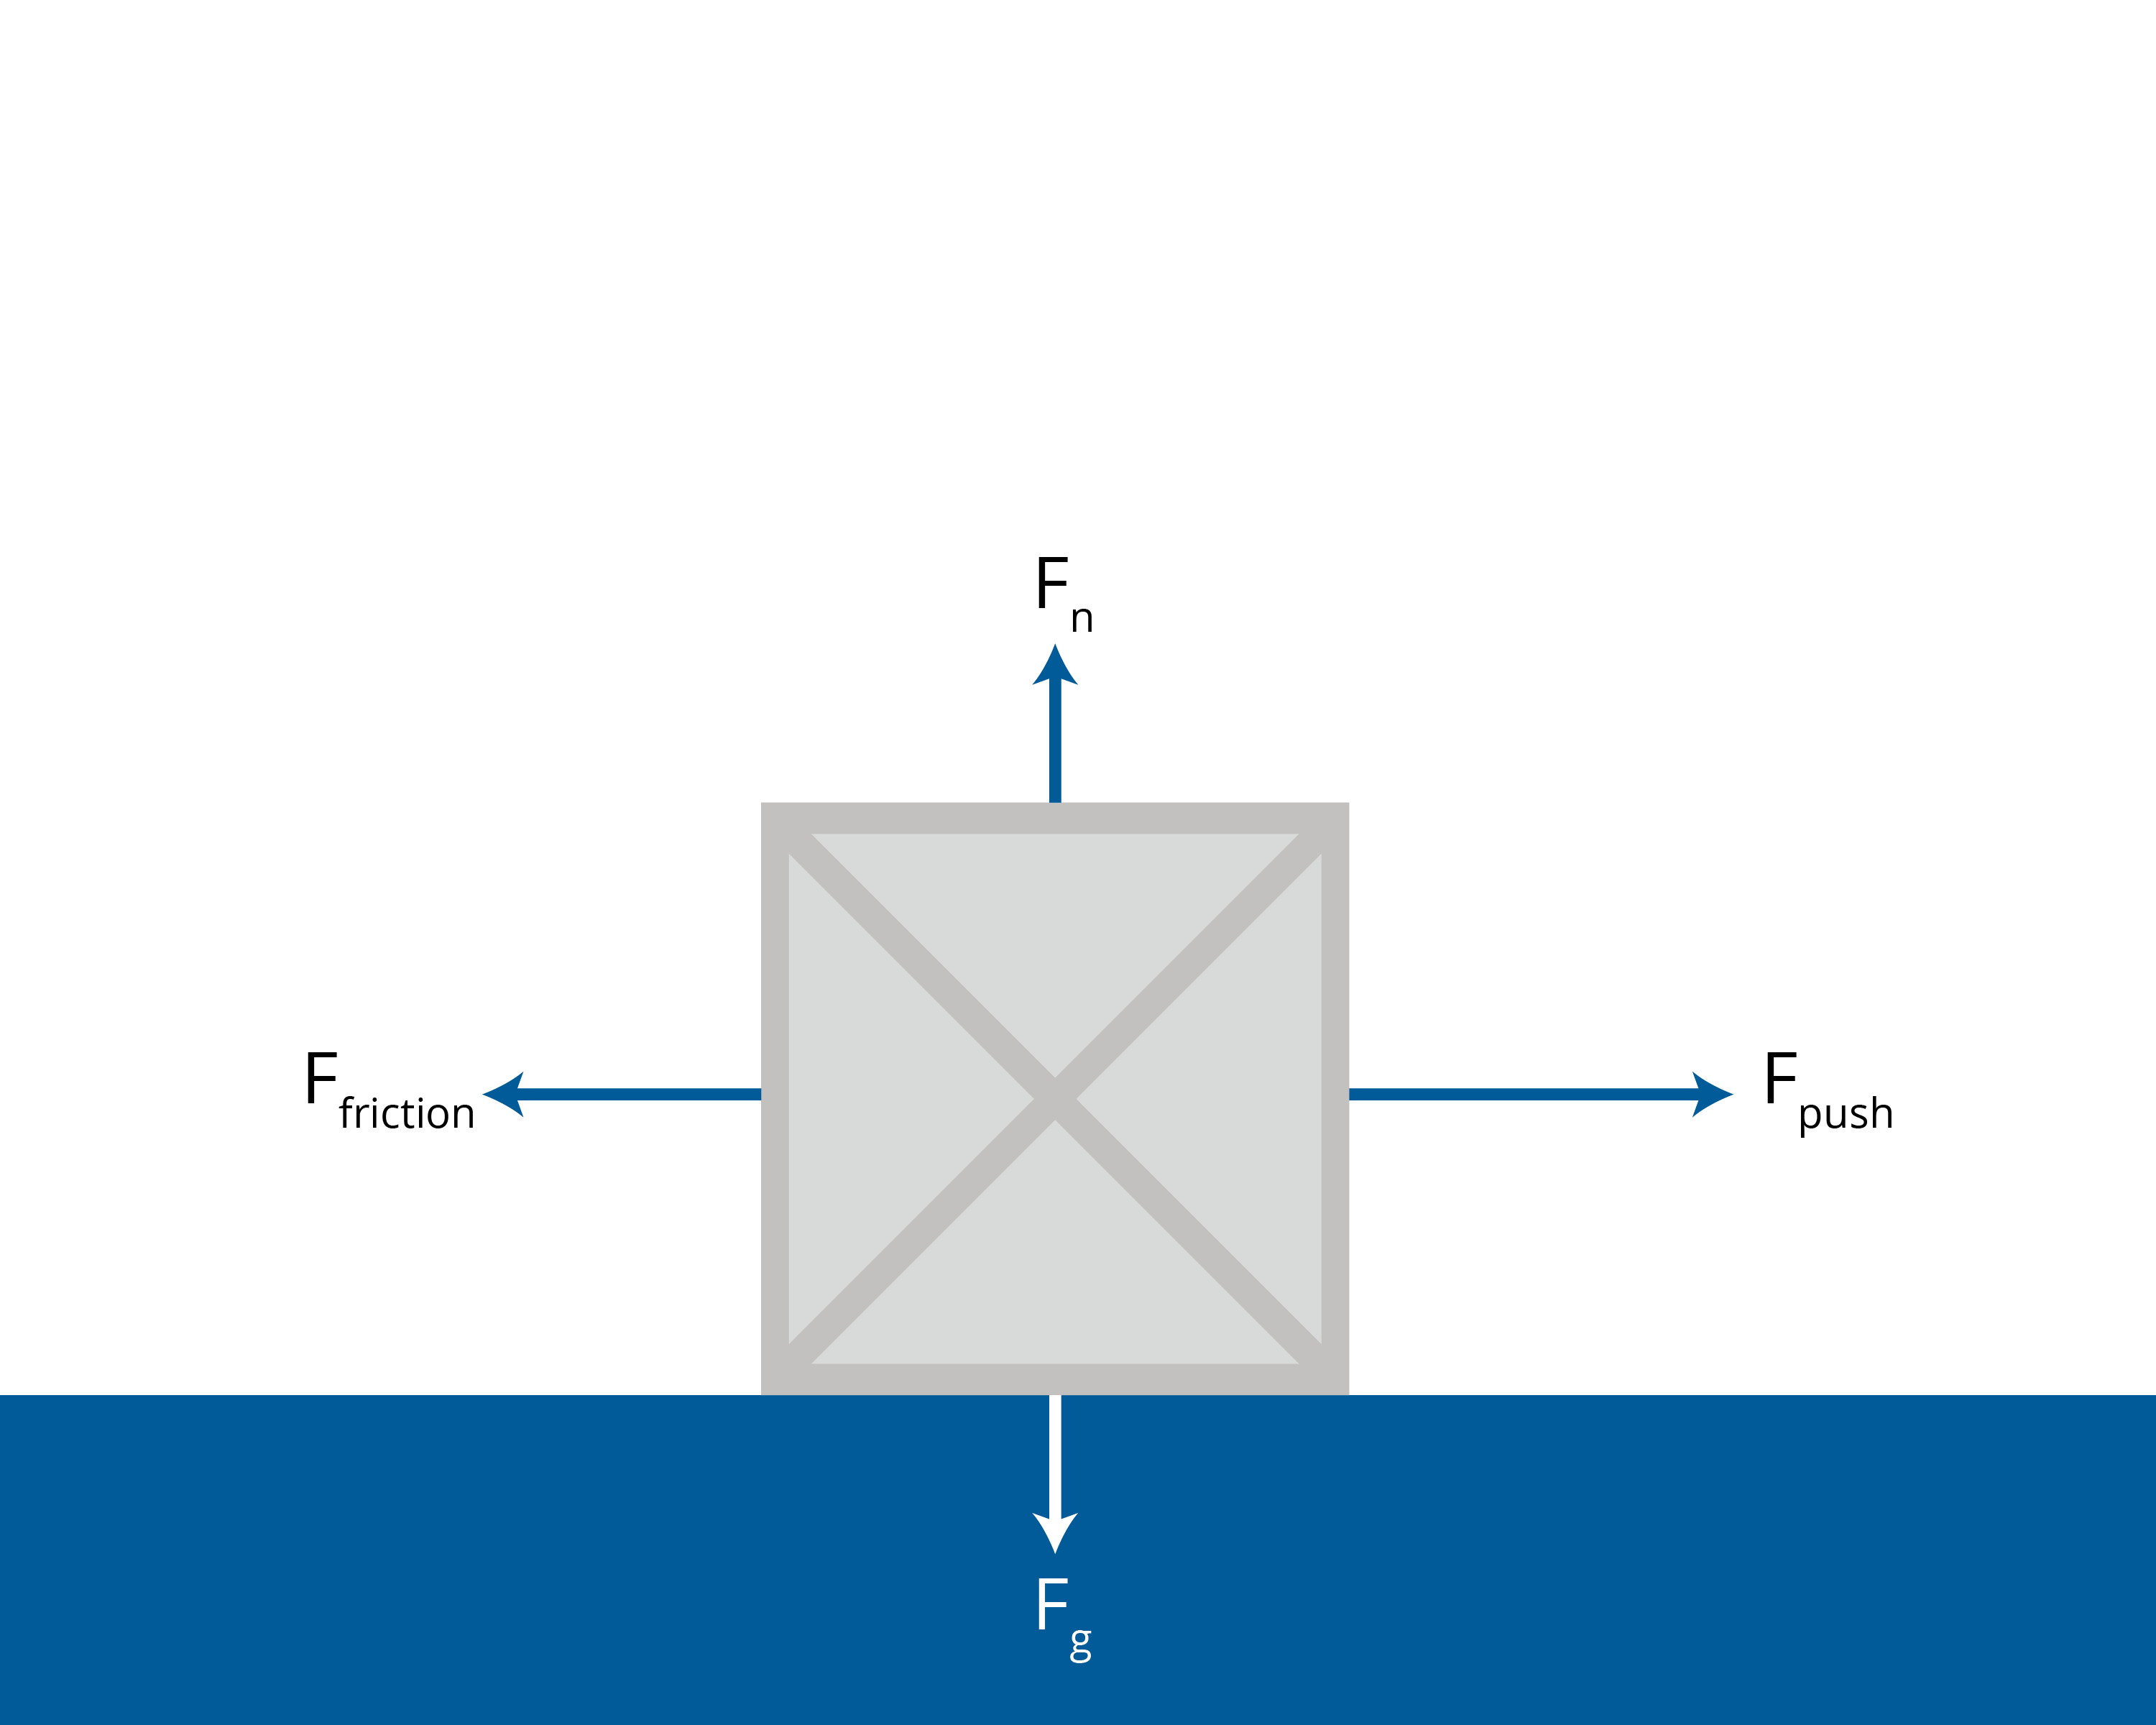
\includegraphics[width=0.75\textwidth]{friction-01.png}
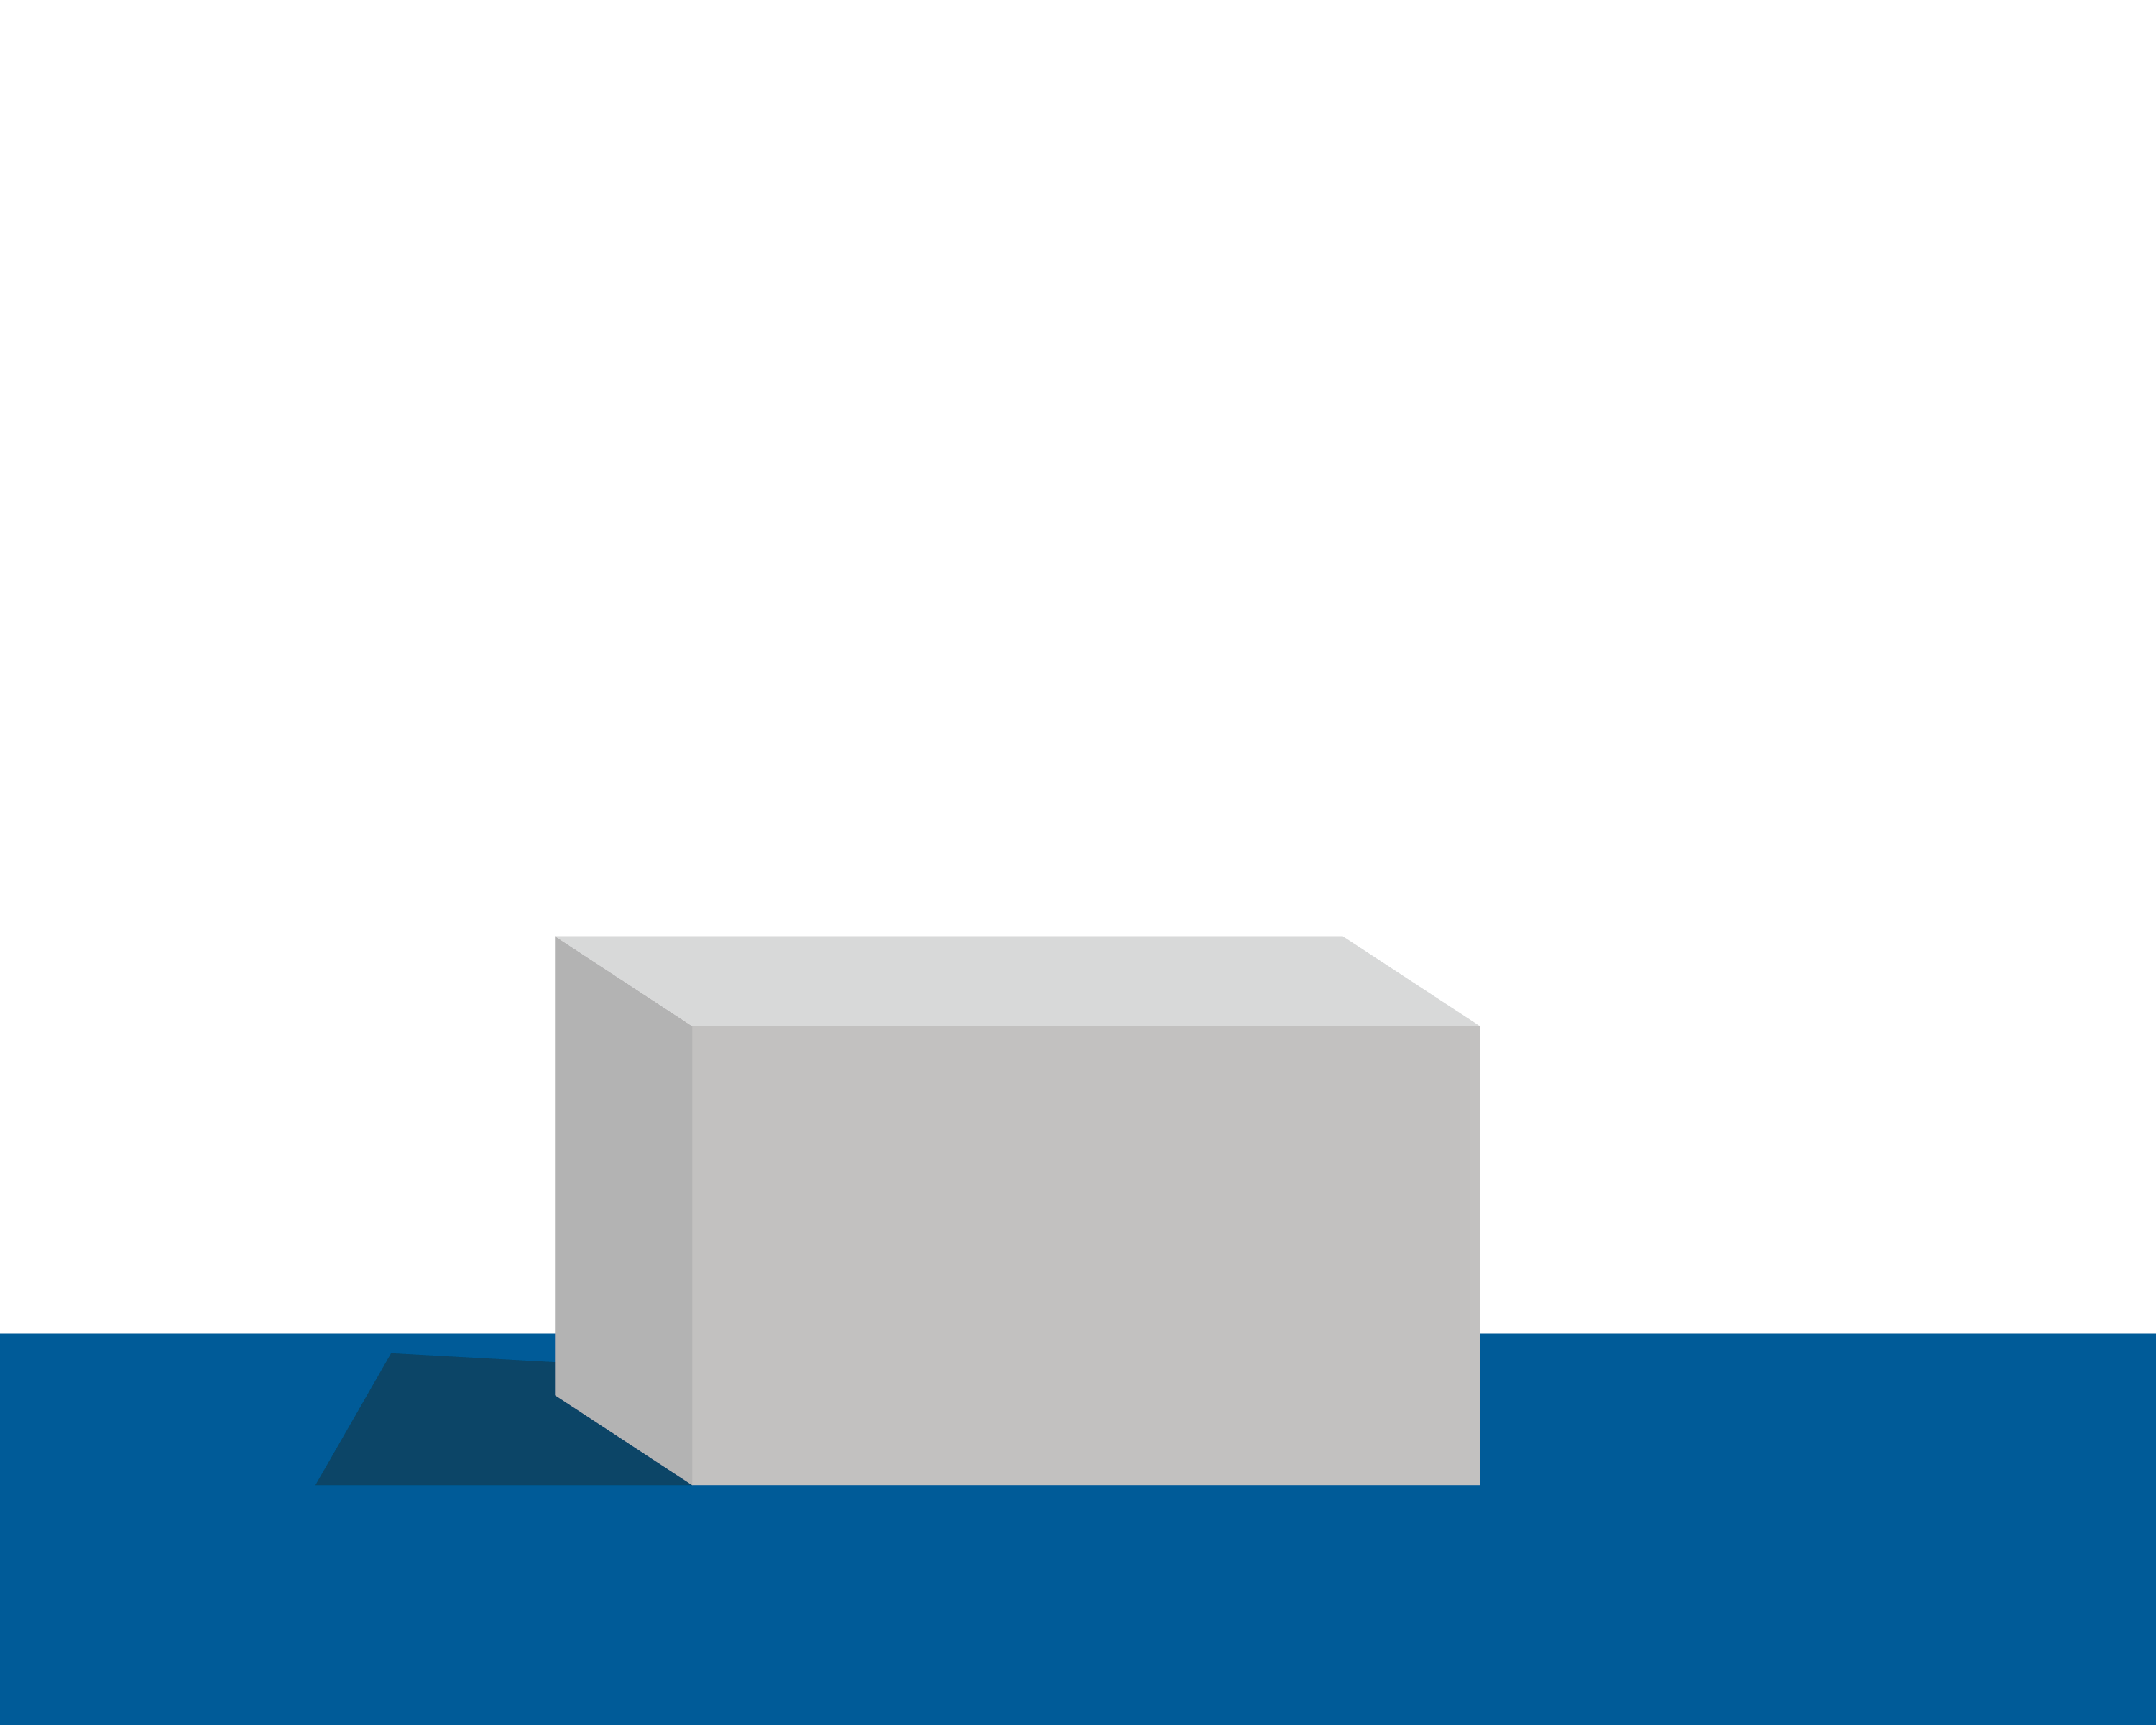
\includegraphics[width=0.75\textwidth]{friction-02.png}
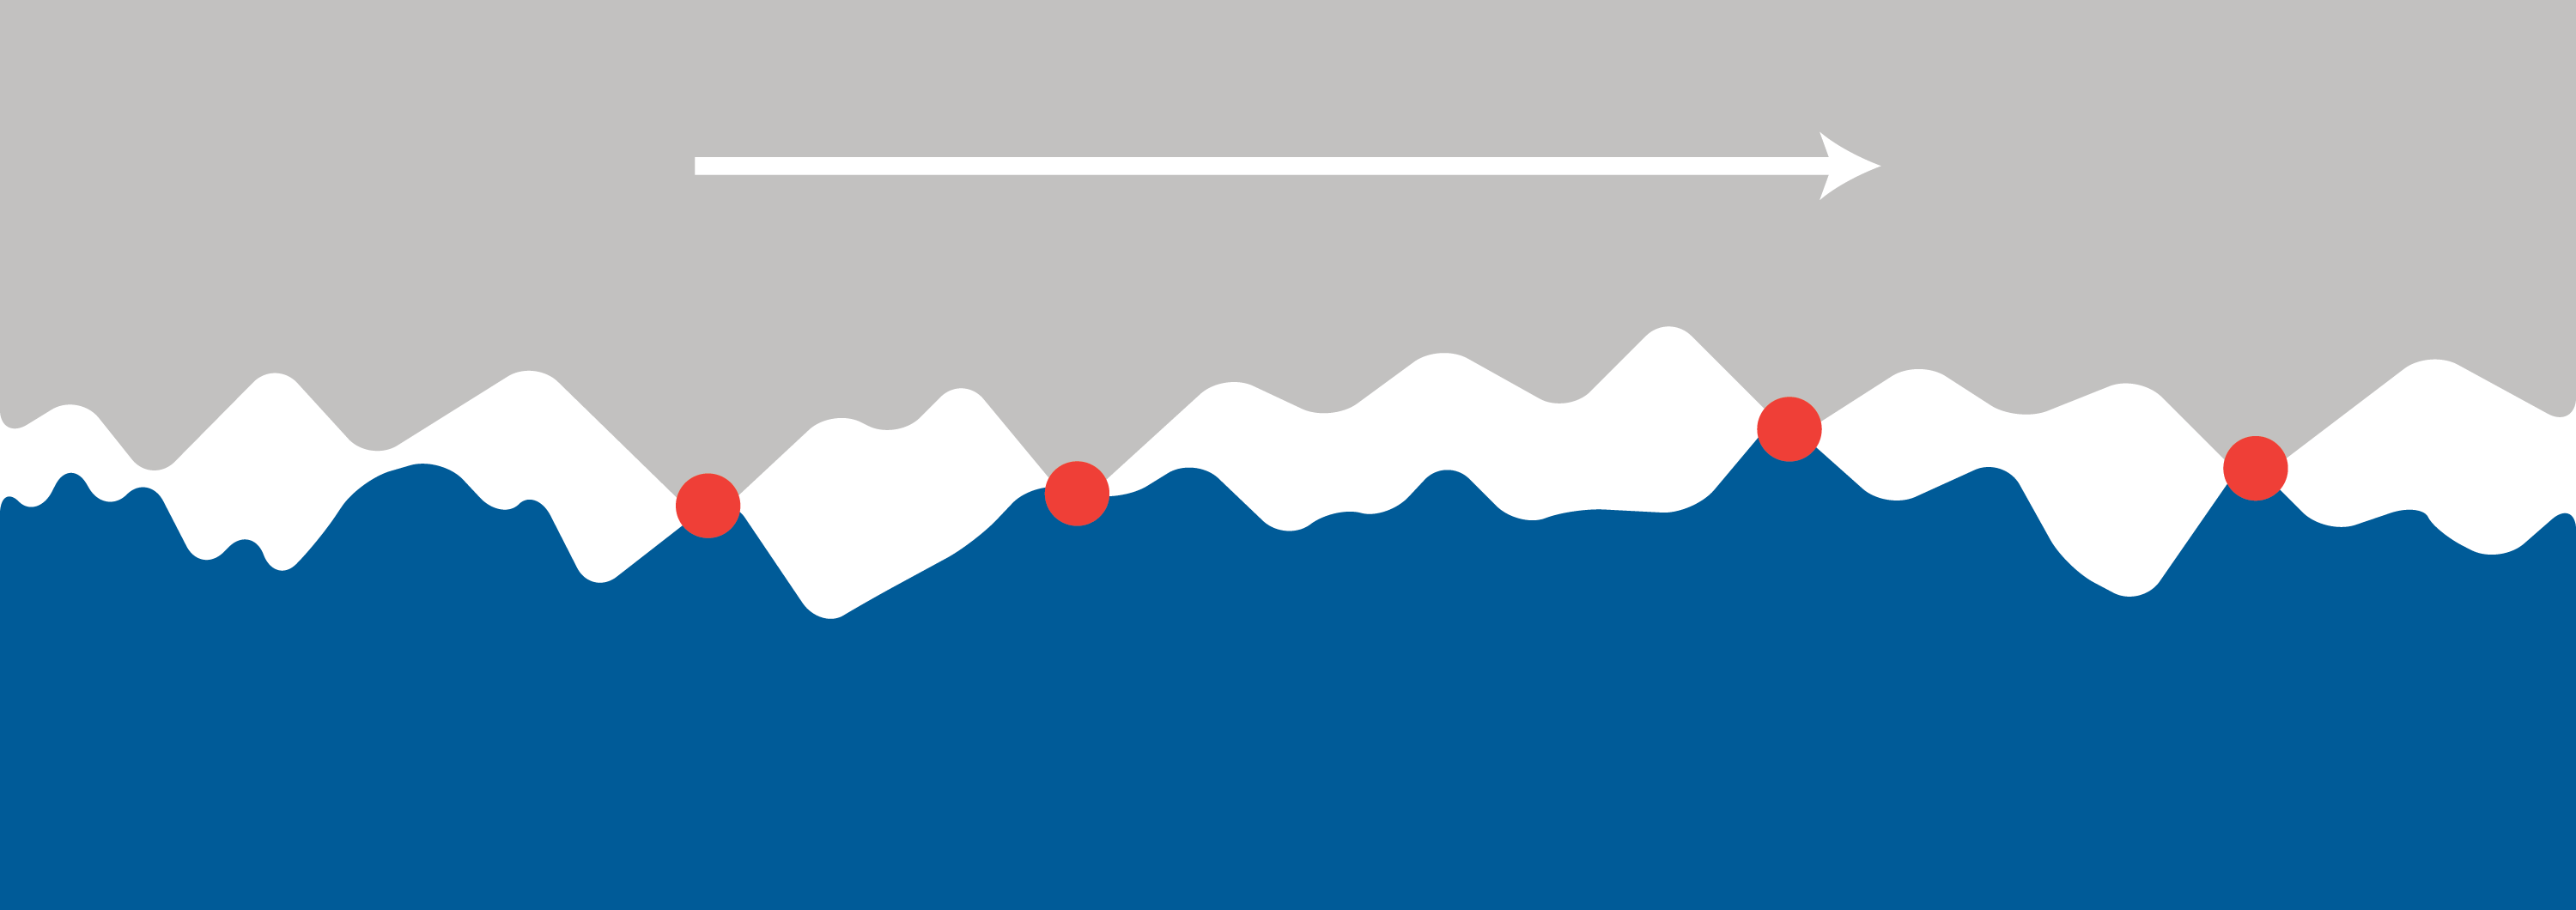
\includegraphics[width=0.75\textwidth]{friction-03.png}
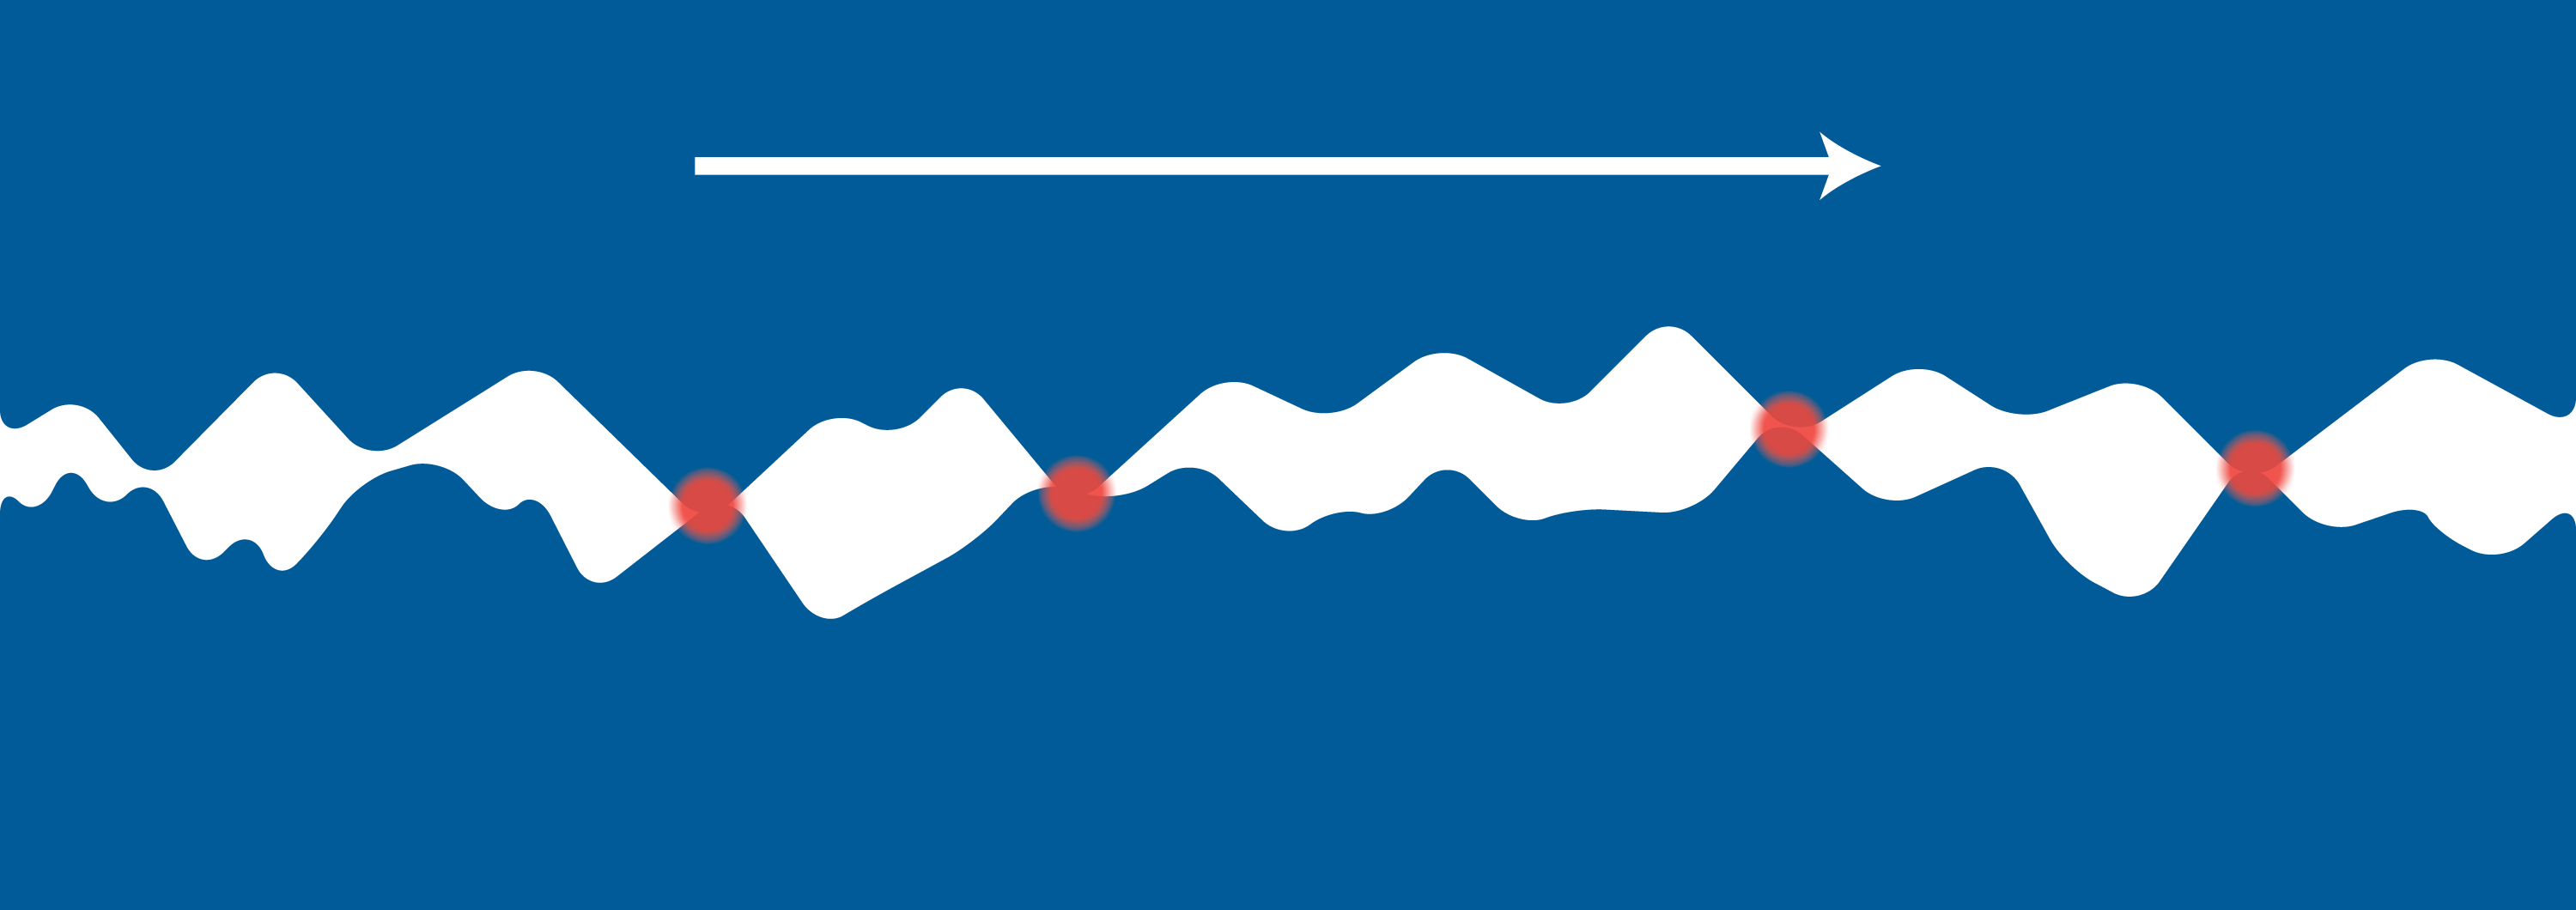
\includegraphics[width=0.75\textwidth]{friction-04.png}
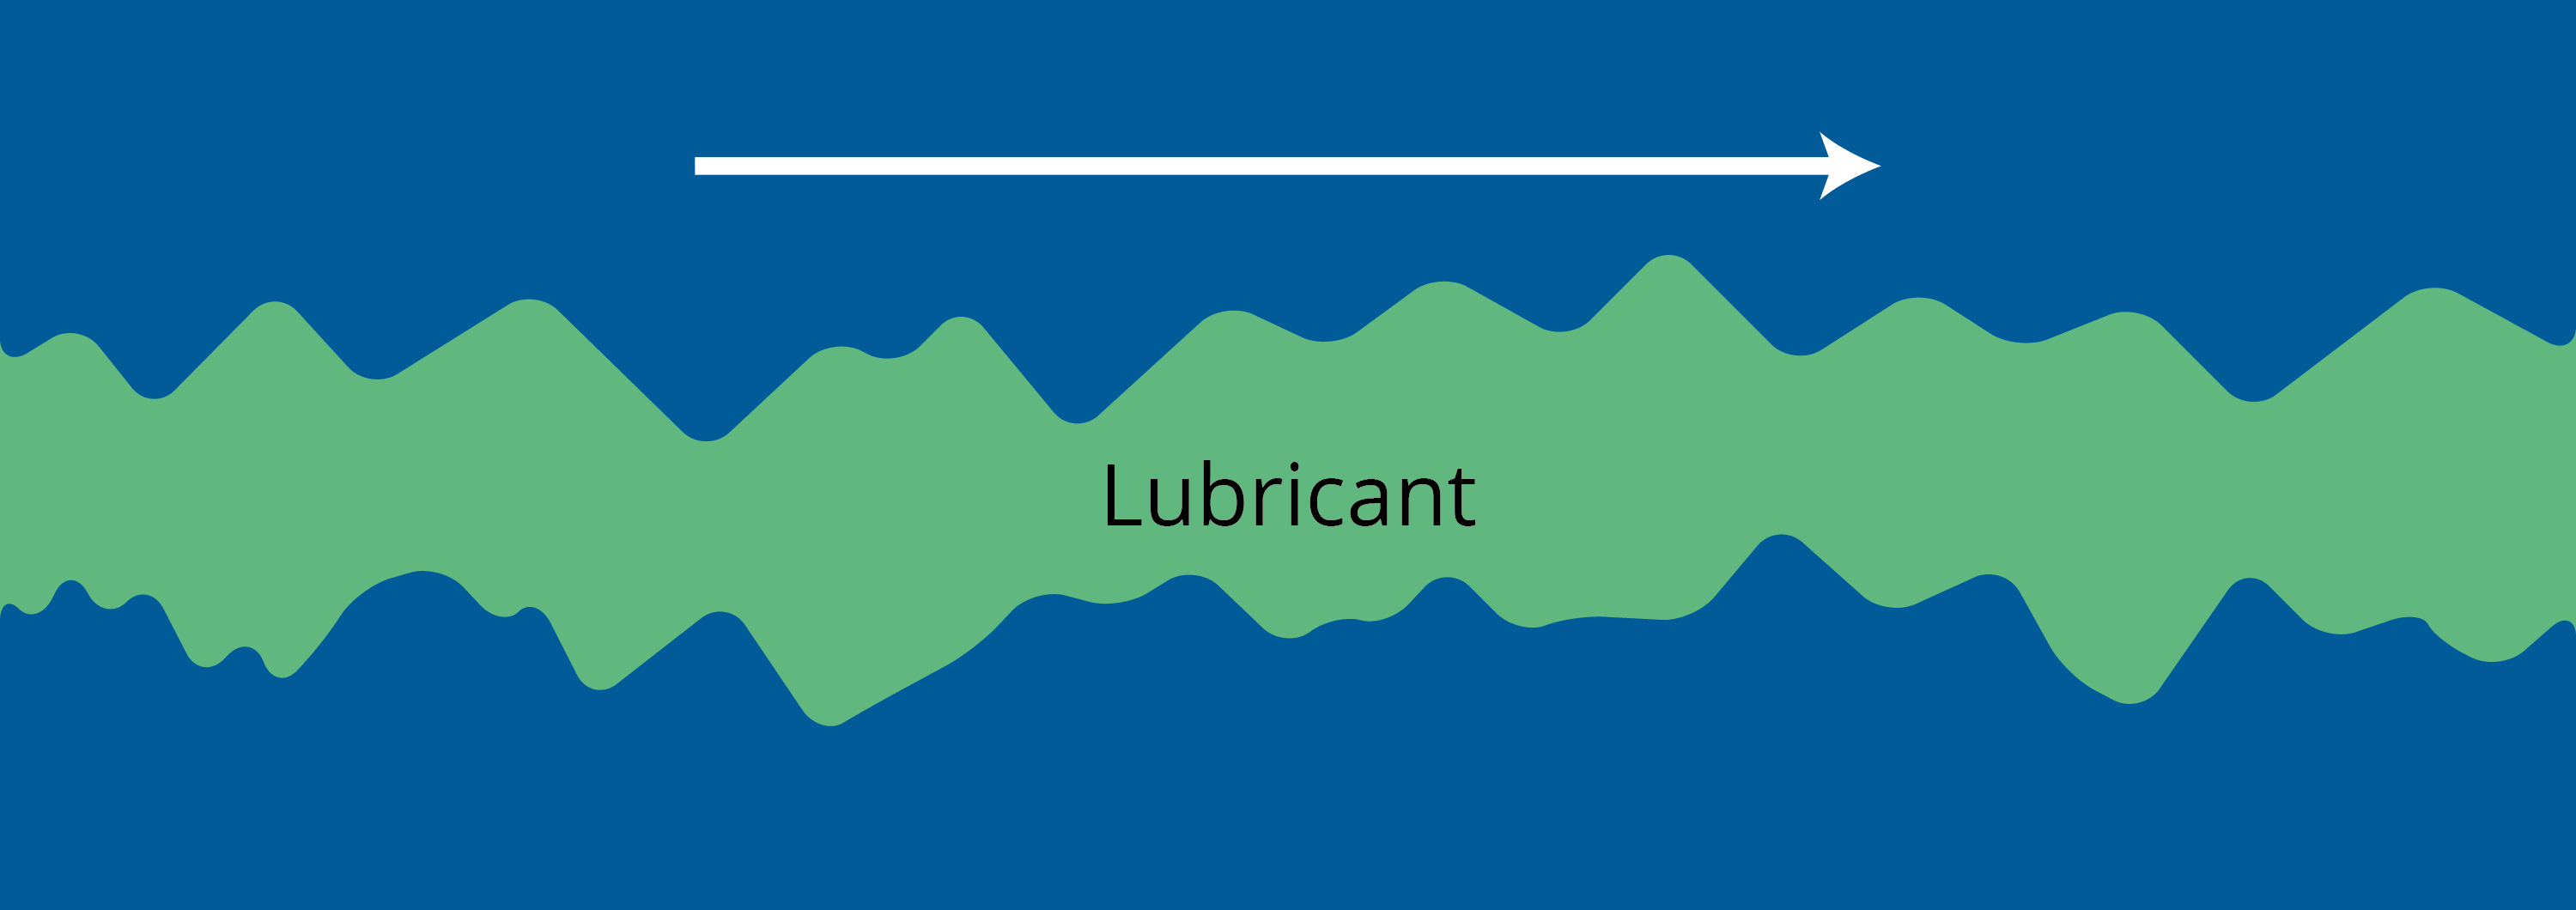
\includegraphics[width=0.75\textwidth]{friction-05.png}
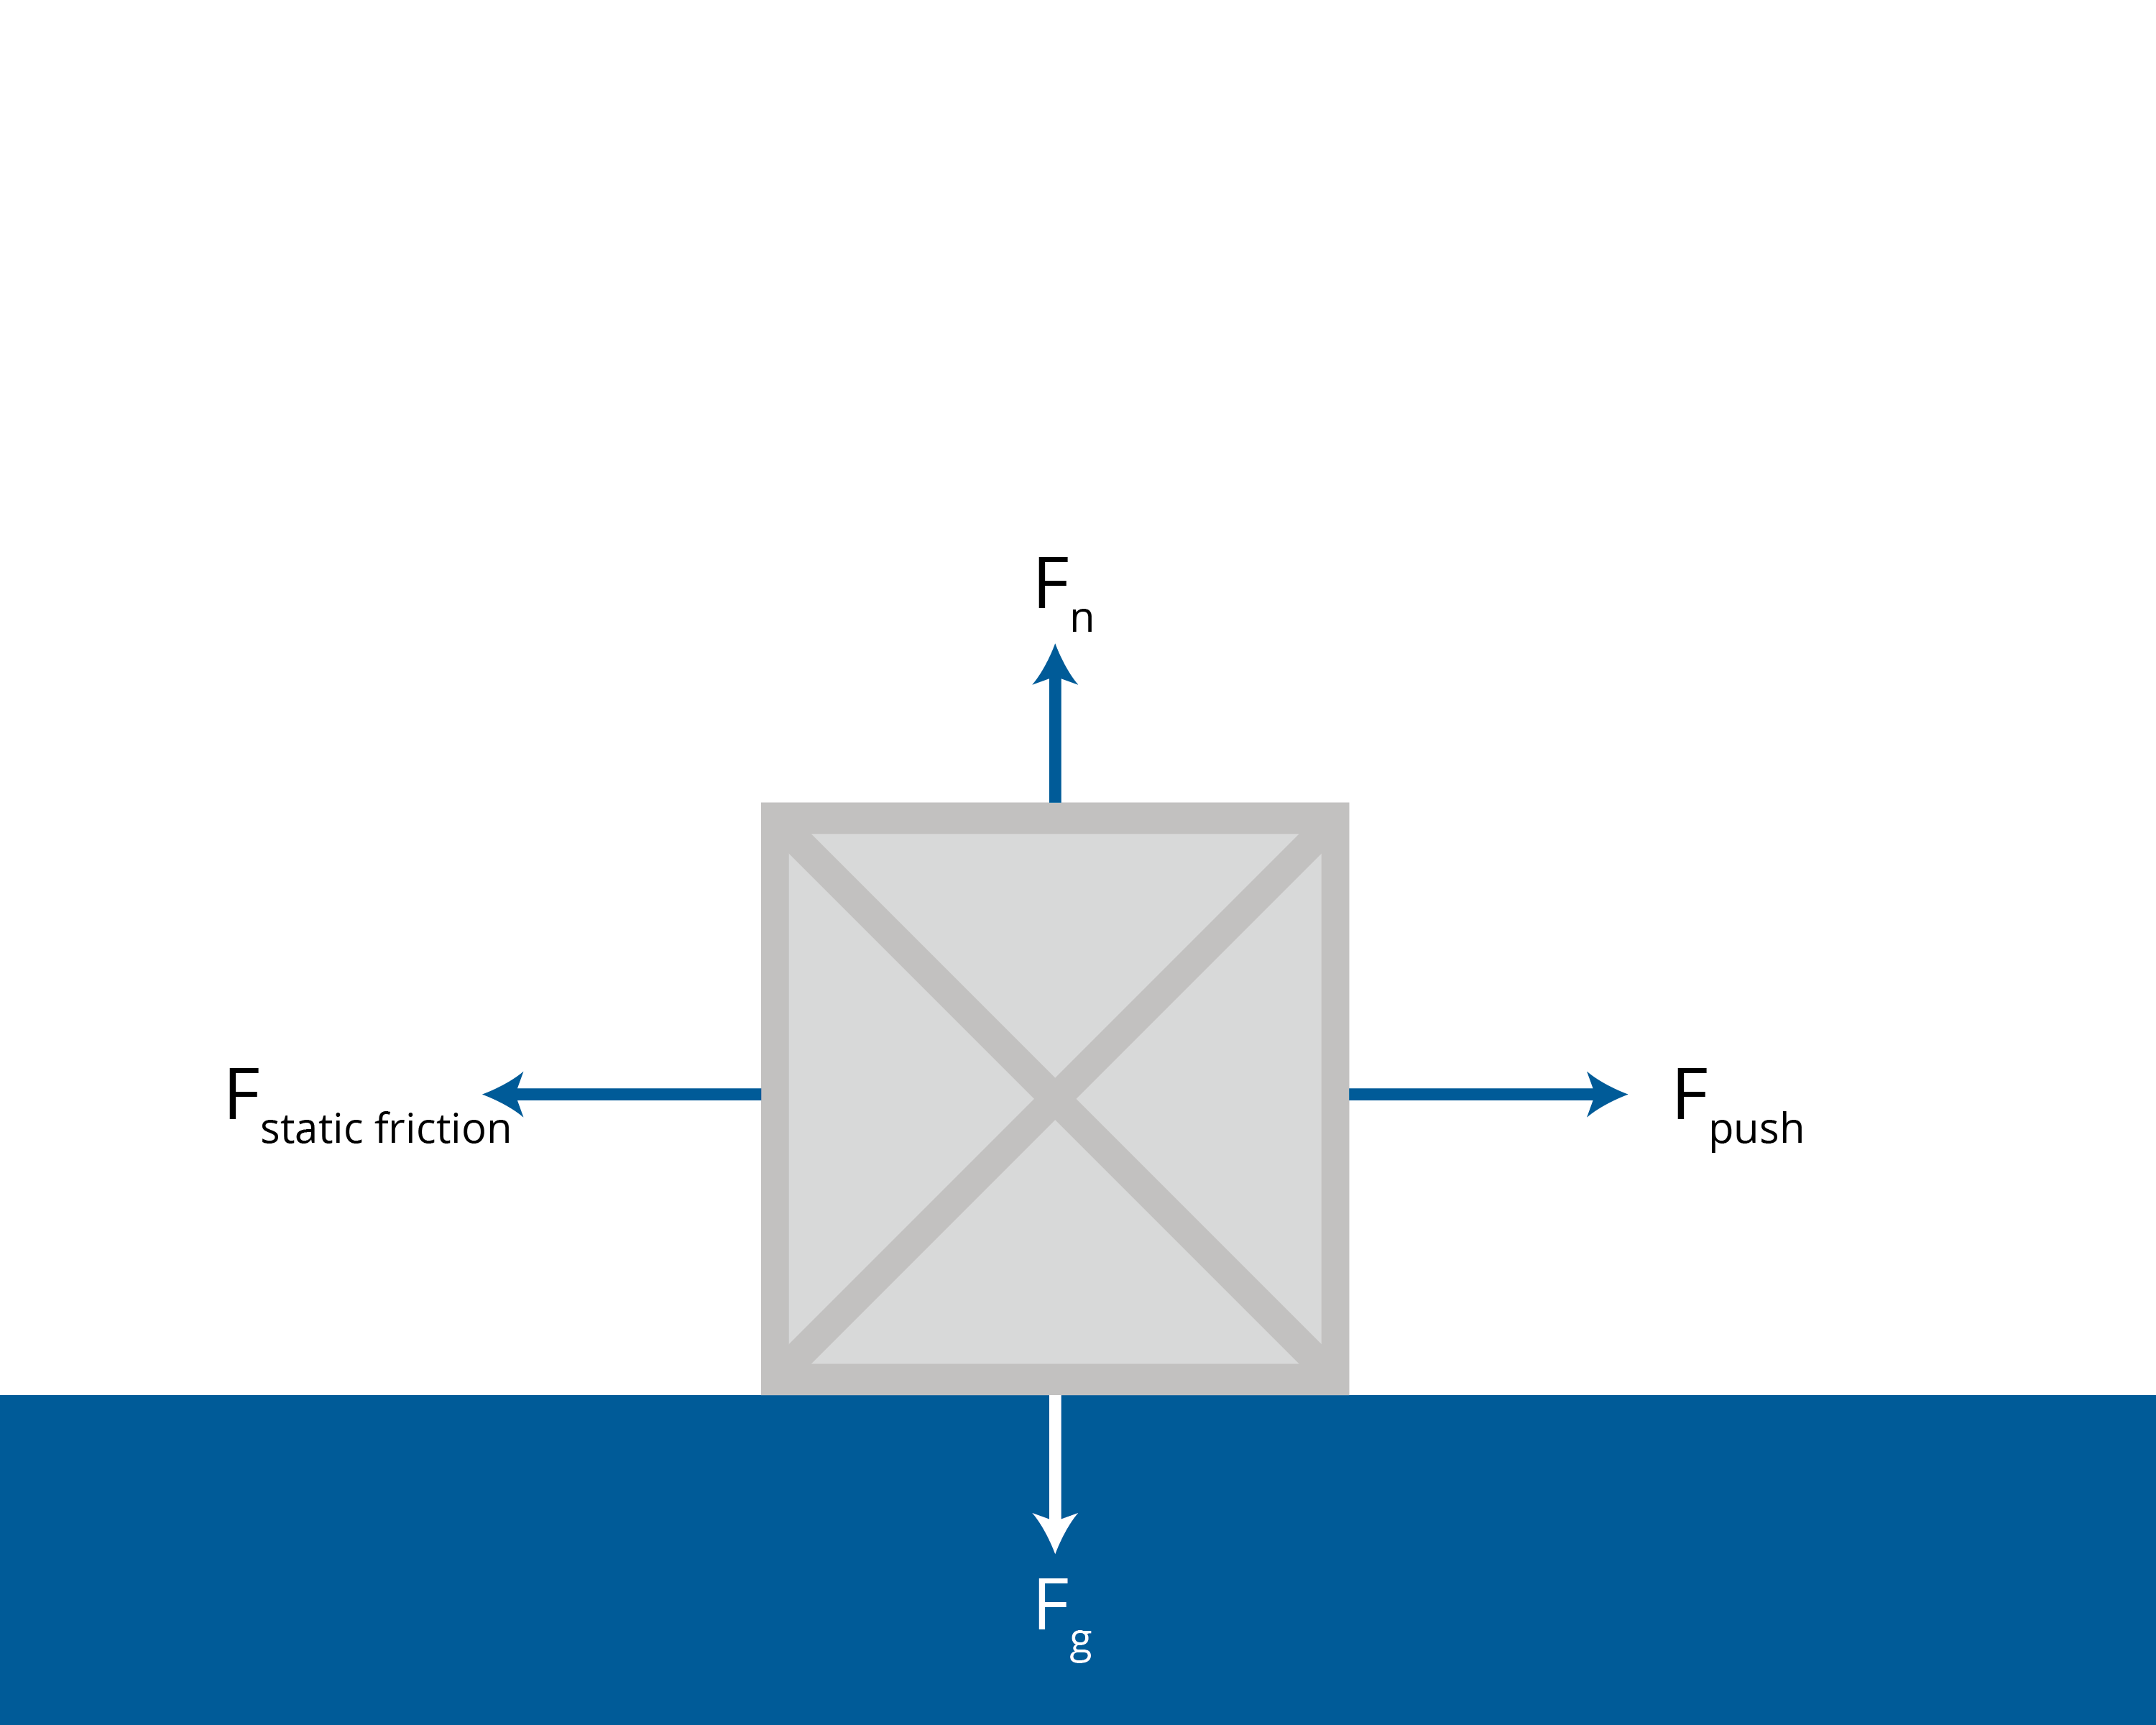
\includegraphics[width=0.75\textwidth]{friction-06.png}
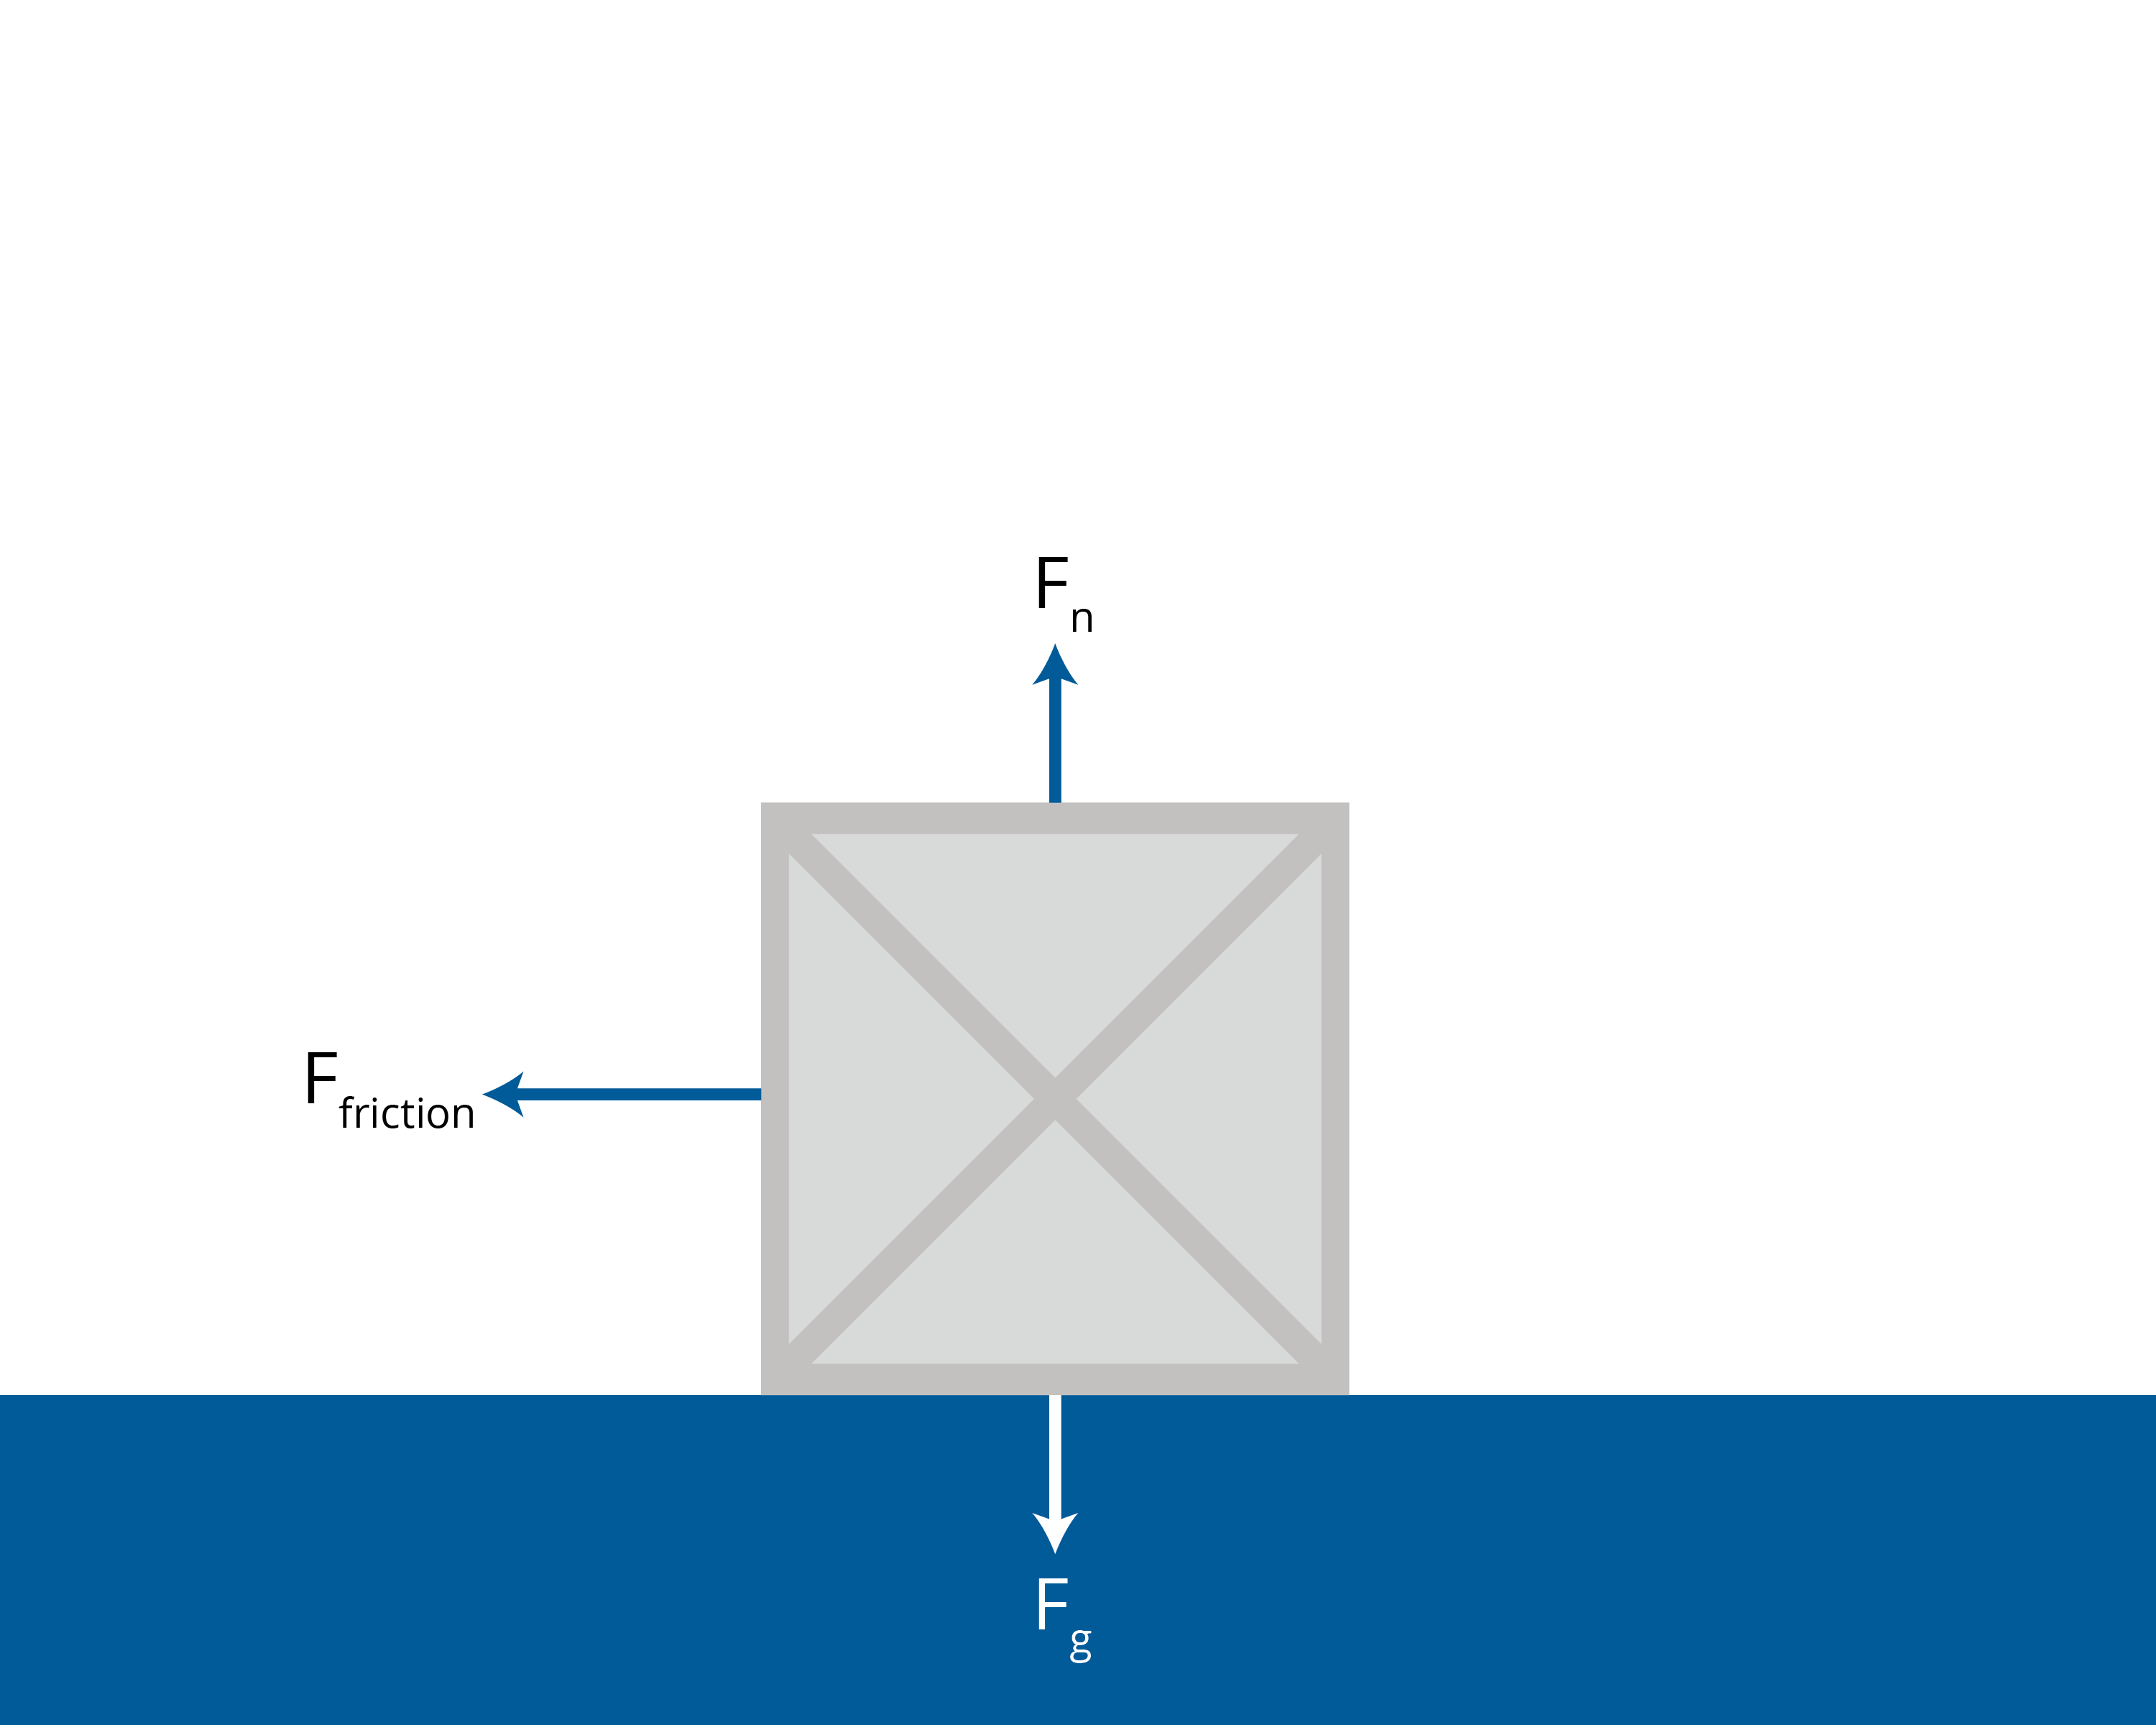
\includegraphics[width=0.75\textwidth]{friction-07.png}








